\documentclass[runningheads]{llncs}

\usepackage{graphicx}
\graphicspath{{./figs/}}

\usepackage{amsmath} 
\usepackage{bm}
\usepackage{amsbsy} 
\usepackage{amssymb}
\usepackage{cite}

\begin{document}
%
\title{Automatic Time Step Selection for Numerical Solution of Neutron Diffusion Problems}
%
%\titlerunning{Abbreviated paper title}
% If the paper title is too long for the running head, you can set
% an abbreviated paper title here
%
\author{A.V. Avvakumov\inst{1} \and
V.F. Strizhov\inst{2}\and
P.N. Vabishchevich\inst{2,3}\and
A.O. Vasilev\inst{3}}
%
\authorrunning{A.V. Avvakumov et al.}
% First names are abbreviated in the running head.
% If there are more than two authors, 'et al.' is used.
%
\institute{National Research Center \emph{Kurchatov Institute}, Moscow, Russia \and
Nuclear Safety Institute of RAS,  Moscow, Russia \and
North-Eastern Federal University, Yakutsk, Russia\\
\email{haska87@gmail.com}
}
%
\maketitle              % typeset the header of the contribution
%
\begin{abstract}
Considering the approximate solution of the boundary value problems for nonstationary equations, the focus should be on the choice of time approximation schemes. 
We propose an algorithm allowing automatic time step evaluation when solving the boundary value problems	for parabolic equations.
The solution is obtained using guaranteed stable implicit schemes, and the step choice is performed with the use of the solution obtained by an explicit scheme.
Formulas for explicit calculation of the time step are derived using the estimation of the approximation error at new time step.
Calculation results obtained for some neutron diffusion problems demonstrate reliability of the proposed algorithm for time step choice. 

\keywords{time step selection \and parabolic equation \and approximation error \and neutron diffusion}
\end{abstract}

\section{Introduction}
For parabolic equations of the second order unconditionally stable schemes are constructed on the basis of implicit approximations \cite{Matus}.
In computational practice two-layer schemes are mostly used, compared with three-layered and multilayered schemes which are not so often used.
The problem of controlling the time step is relatively well worked out for an approximate solution of the Cauchy problem for systems of differential equations \cite{Ascher}. 
The main approach is that on the basis of additional calculations, the error of the approximate solution is estimated at a new time step. 
The step is estimated from the theoretical asymptotic dependence of the accuracy on time step and after that correction of step is applied, if necessary, the calculations are repeated \cite{Vabishchevich}.

The algorithm takes into account the features of neutron diffusion problems \cite{Lozenets16}, for instance, fast changes in the solution or instability with respect to the initial data. When using the algorithm, we can expect a noticeable saving in calculation time compared with the fine mesh calculation, while maintaining the required accuracy of the calculation.

\section{Problem description}
Consider the Cauchy problem for the linear equation
\begin{equation}\label{1}
\frac{du}{dt} + A(t)u =f(t), \quad 0 < t \leq T,
\end{equation}
with initial condition $u(0) = u^0$.

The problem is considered in a finite-dimensional Hilbert space.
We assume that $A(t) \geq 0$.
Introduce irregular time grid
\[
t^0 = 0, \quad t^{n+1} = t^n + \tau^{n+1}, \quad 
n = 0, 1, ... , N-1, \quad t^N = T.
\]
For approximate solution the implicit scheme are used
\begin{equation}\label{3}
\begin{split}
  \frac{y^{n+1} - y^{n}}{\tau^{n+1}} + A^{n+1} y^{n+1} = f^{n+1},
  \quad n = 0,1, ..., N-1, 
\end{split}
\end{equation}
and initial condition 
$
y^0 = u^0 .
$
For an approximate solution under constraints follows a layerwise estimate
\[
 \|y^{n+1}\| \leq \|y^{n}\| + \tau^{n+1} \|f^{n+1}\| .
\]
Then we obtain a difference estimate
\begin{equation}\label{5}
 \|y^{n+1}\| \leq \|u^{0}\| + \sum_{k=0}^{n} \tau^{k+1} \|f^{k+1}\|
\end{equation}
for problem (\ref{3}).
For the error of the approximate solution $z^n = y^n - u^n$ we have
\[
  \frac{z^{n+1} - z^{n}}{\tau^{n+1}} + A^{n+1} z^{n+1} = \psi^{n+1},
  \quad n = 0,1, ..., N-1,  \quad
 z^0 = 0.
\]
Here $\psi^{n+1}$ is approximation error
\begin{equation}\label{6}
 \psi^{n+1} = f^{n+1} -
 \frac{u^{n+1} - u^{n}}{\tau^{n+1}} - A^{n+1} u^{n+1} . 
\end{equation}
Similarly (\ref{5}) we have an estimate for the error
\begin{equation}\label{7}
  \|z^{n+1}\| \leq \sum_{k=0}^{n} \tau^{k+1} \|\psi^{k+1}\| .
\end{equation} 
Checking the error we can focus on the total error $\delta\tau^{n+1}$ in interval $t^n < t < t^{n+1}$. Then from (\ref{7}) we obtain
$\|z^{n+1}\| \leq \delta t^{n+1}.$
The error accumulates and increases linearly.

The solution is obtained using guaranteed stable implicit schemes.
This scheme includes main computing costs.
The step choice is performed with the use of the solution obtained by the explicit scheme.
The stability of our algorithm is not violated. 
It is determined by the properties of the implicit scheme.

The accumulation of errors in the transition from the time layer $t^n$ to the new layer $t^{n+1}$  is defined as
\begin{equation}\label{8}
\|z^{n+1}\| \leq \|z^{n}\| + \tau^{n+1} \|\psi^{n+1}\| .
\end{equation}
Therefore, we must control the local error $\psi^{n+1}$. Comparing $\psi^{n+1}$ with a given level of error $\delta$ we can judge the quality of the time step choice. If $\psi^{n+1}$ is significantly larger (smaller) then the $\delta$ that the time step is taken too large (small). Thereby
\begin{equation}\label{9}
  \tau^{n+1}: \ \|\psi^{n+1}\| \approx \delta .
\end{equation} 

Consider the main algorithm for choosing the time step. We select the predicted step in time based on the analysis of the solution at the previous steps in time. The predicted time step is determined as following
\begin{equation}
 \widetilde{\tau}^{n+1} = \gamma \tau^n , 
\end{equation}
where $\gamma$ is numeric parameter. The default parameter of $\gamma$ is 1.25 or 1.5. Using the explicit scheme we find a solution $\widetilde{y}^{n+1}$ at time $\widetilde{t}^{n+1} = t^n + \widetilde{\tau}^{n+1}$. The calculation is done only on one step in time therefore the possible computational instability does not appear.
We estimate the error of approximation by the found $\widetilde{y}^{n+1}$ using the implicit scheme. The $\tau^{n+1}$ is estimated by the closeness of the error norm to $\delta$. The solution at a new time step $t^{n+1}$ is calculated with a $\tau^{n+1}$  by a implicit scheme.

\section{Calculated formulas}
We present the calculated formulas for the choice of the time step for the neutron diffusion equation.

\textbf{Neutron diffusion equation.}
Let's consider modelling neutron flux in a one group diffusion approximation with one group delayed neutron sources. Neutron flux dynamics is considered within a bounded 2D domain  $\Omega$ ($\bm x = \{x_1, x_2\} \in \Omega$) with a convex boundary $\partial \Omega$.
 \begin{equation}\label{11}
\begin{split}
 \frac{1}{v} \frac{\partial \phi}{\partial t} -  \nabla \cdot D \nabla \phi + \Sigma_{a} \phi &=   \ (1-\beta) \nu \Sigma_{f} \phi + \lambda c, \\
\frac{\partial c}{\partial t} + \lambda c &= \beta \nu \Sigma_{f} \phi.
\end{split}
\end{equation} 
Here $\phi(\bm x,t)$ is the neutron flux at point $\bm x$ and time $t$,
$v$ is the effective velocity of neutrons,
$D(\bm x)$ is the diffusion coefficient, 
$\Sigma_{a}(\bm x,t)$ is the absorption cross-section,
$\beta$ is the effective fraction of delayed neutrons, 
$\nu\Sigma_{fg}(\bm x,t)$ is the generation cross-section,
$c$ is density of source of delayed neutrons, 
$\lambda$  is decay constant of source of delayed neutrons.

The conditions so-called albedo-type are set at the boundary $\partial \Omega$:
\begin{equation}\label{12}
 D\frac{\partial \phi}{\partial n} + \gamma \phi = 0.
\end{equation}\label{13}
where $n$ is the outer normal to the boundary $\partial \Omega$.
Let's consider problem (\ref{11}) with boundary conditions (\ref{12}) and initial conditions:
$
 \phi(0) = \phi^0,  \,
 c(0) = c^0.
$
Space discretization is performed using the standard Lagrange finite elements (for example, see \cite{Matmod}).

\textbf{Time step estimate.}
In our case, the approximation error $\bm{\psi^{n+1}} = \{\psi^{n+1}_1, \psi^{n+1}_2\}$ is
\begin{equation}\label{14}
\begin{split}
\psi^{n+1}_1  & =  \frac{1}{v} \frac{\phi^{n+1}-\phi^n}{\tau^{n+1}} - \nabla \cdot D^{n+1} \nabla \phi^{n+1} + \Sigma_{a}^{n+1} \phi^{n+1} \\
 & - (1-\beta) \nu \Sigma^{n+1}_{f} \phi^{n+1} - \lambda  c^{n+1}, \\
\psi^{n+1}_2  & =  \frac{ c^{n+1}-c^n}{\tau^{n+1}} + \lambda c^{n+1} - \beta \nu\Sigma_{f}^{n+1} \phi^{n+1},
\end{split}
\end{equation} 
where $\bm{\phi^{n+1}} = \{ \phi^{n+1}, c^{n+1} \}$ is exact solution.
The predictive solution is 
\begin{equation}\label{15}
\begin{split}
\frac{1}{v} \frac{\widetilde\varphi^{n+1}-\varphi^n}{\widetilde\tau^{n+1}} - \nabla \cdot D^n \nabla \varphi^n + \Sigma^n_{a} \varphi^n & = (1-\beta) \nu \Sigma^n_{f} \varphi^n + \lambda s^n, \\
\frac{\widetilde s^{n+1}-s^n}{\widetilde\tau^{n+1}} + \lambda s^n &= \beta \nu\Sigma^n_{f} \varphi^n.
\end{split}
\end{equation} 
This solution is used to estimate the approximation error of the implicit scheme in the transition from time $t^n$ to time $\widetilde{t}^{n+1}$.

In accordance with (\ref{14}), the approximation error is calculated from the exact solution for two moment of time: in our case for $t^n$ and $\widetilde{t}^{n+1}$.
To estimate the error, it is necessary to match something between $\bm{\phi}(t^n)$ and $\bm{\phi}(\widetilde{t}^{n+1})$.  We take $\bm{\varphi^n} = \{\varphi^n, s^n\}$ instead of $\bm{\phi}(t^n)$. To an exact solution on a new layer $\bm{\phi}(\widetilde{t}^{n+1})$, we match an approximate solution $\bm{\widetilde{\varphi}^{n+1}} = \{\widetilde{\varphi}^{n+1}, \widetilde{s}^{n+1}\}$, which is obtained by the explicit scheme. In view of this, we set
\begin{equation}\label{16}
\begin{split}
\widetilde\psi^{n+1}_1  & =  \frac{1}{v} \frac{\widetilde\varphi^{n+1}-\varphi^n}{\widetilde\tau^{n+1}} - \nabla \cdot D^{n+1} \nabla \widetilde\varphi^{n+1} + \Sigma_{a}^{n+1} \widetilde\varphi^{n+1} \\
&- (1-\beta) \nu \Sigma^{n+1}_{f} \widetilde\varphi^{n+1} - \lambda \widetilde s^{n+1}, \\
\widetilde\psi^{n+1}_2  & =  \frac{\widetilde s^{n+1}-s^n}{\widetilde\tau^{n+1}} + \lambda \widetilde s^{n+1} - \beta \nu\Sigma_{f}^{n+1} \widetilde\varphi^{n+1}.
\end{split}
\end{equation} 
We match the approximation error $\bm{\widetilde{\psi}^{n+1} }= \{\widetilde{\psi}^{n+1}_1, \widetilde{\psi}^{n+1}_2\}$ with the time step $\widetilde{\tau}^{n+1}$ and $\bm{\psi^{n+1}}$ with the time step $\tau^{n+1}$.
Taking into account (\ref{9}), we set
\begin{equation}\label{17}
  \bar{\tau}^{n+1} = \gamma_{n+1} \tau^n,
  \quad \gamma_{n+1} = \frac{\delta}{\| \bm{\widetilde{\psi}^{n+1}}\|}  \gamma.
\end{equation} 
The needed time step can not exceed the predicted time step, therefore
\[
\tau^{n+1} \leq \bar{\tau}_{n+1}, \quad \tau^{n+1} \leq \widetilde{\tau}_{n+1}.
\] 
We limit the allowable time step by the minimum step $\tau^0$:
\begin{equation}\label{18}
 \tau^{n+1} = \max \big \{\tau^0, \min \{\gamma_{n+1}, \gamma \} \tau^n \big \}. 
\end{equation}
Let's determine  the calculation formulas for the step selection algorithm in accordance with (\ref{15})-(\ref{18}):
\[
 \begin{split}
 \widetilde{\psi}^{n+1}_1  &  =  (- \nabla \cdot D^{n+1} \nabla  + \Sigma_{a}^{n+1}  - (1-\beta) \nu \Sigma^{n+1}_{f}  + \nabla \cdot D^n \nabla - \Sigma^n_{a} + (1-\beta) \nu \Sigma^n_{f}) \varphi^{n} \\
& + (- \nabla \cdot D^{n+1} \nabla  + \Sigma_{a}^{n+1}  - (1-\beta) \nu \Sigma^{n+1}_{f}) (\widetilde{\varphi}^{n+1} - \varphi^n) - \lambda (\widetilde{s}^{n+1} - s^n).\\
 \widetilde{\psi}^{n+1}_2 &  =   (-\beta\nu\Sigma^{n+1}_f + \beta\nu\Sigma^{n}_f)\varphi^n + \lambda (\widetilde s^{n+1} - s^n) - \beta\nu\Sigma^{n+1}_f (\widetilde\varphi^{n+1} - \varphi^n) .
 \end{split} 
\] 
For convenience, rewrite it in the operator notation
\[
\begin{split}
\bm{\widetilde{\psi}^{n+1}} &= (A^{n+1} - A^n)\bm{\varphi^n} + {A}^{n+1}(\bm{\widetilde{\varphi}^{n+1}} - \bm{\varphi^n}) \\
&= \widetilde{\tau}^{n+1} \left( \frac{A^{n+1} - A^n}{\widetilde{\tau}^{n+1}} \bm{\varphi^n} + A^{n+1} \frac{\bm{\widetilde{\varphi}^{n+1}} - \bm{\varphi^n}}{\widetilde{\tau}^{n+1}} \right),
\end{split}
\]
where 
\[
\begin{split}
A &= \begin{pmatrix}
  - \nabla \cdot D \nabla  + \Sigma_{a}  - (1-\beta) \nu \Sigma_{f} - \lambda & 0  \\
  0  & \lambda - \beta\nu\Sigma_f   \\
 \end{pmatrix}.
\end{split} 
\]
Thus, the approximation error has the first order in
time:
$
\bm{\widetilde{\psi}^{n+1}} = \mathcal{O} (\widetilde{\tau}_{n+1}).
$
In view of this, we set 
\begin{equation}\label{19}
 \|\bm{\widetilde{\psi}^{n+1}} \| \leq \| (A^{n+1} - A^n) \bm{\varphi^n} +
 A^{n+1} (\bm{\widetilde{\varphi}^{n+1}} - \bm{\varphi^n}) \| .
\end{equation} 
Taking into account (\ref{19})  from (\ref{17}), we obtain the calculated formula for time step (\ref{18}), in which
\begin{equation}\label{20}
  \gamma_{n+1} = \frac{\delta}{ \| (A^{n+1} - A^n) \bm{\varphi^n}  +
  A^{n+1} (\bm{\widetilde{\varphi}^{n+1}} - \bm{\varphi^n}) \| } \gamma .
\end{equation}
In this formula (the denominator of the expression), the corrective actions for selecting the time step are clearly reflected, which are associated with the change of the problem operator (the first part), with the dynamics of the solution (second part).

\section{Test problem}
The test problem for reactor IAEA-2D without a reflector in a one-dimensional approximation ($\Omega$ --- is the reactor core area) is considered \cite{Chao}. The geometrical model of the IAEA-2D reactor core is presented in Fig.\ref{fig:1}. The fuel assembly pitch equals 20 cm. Diffusion neutronics constants in the common notations are given in Table \ref{t-1}. 
The boundary conditions (\ref{3}) are used at $\gamma_g = 0.5$.
The following delayed neutrons parameters are used: $\beta = 6.5 \cdot 10^{−3}$, $\lambda = 0.08$ s$^{-1}$ and $v = 1.0 \cdot 10^6$ cm/s.
\begin{figure}[ht]
  \begin{center}
    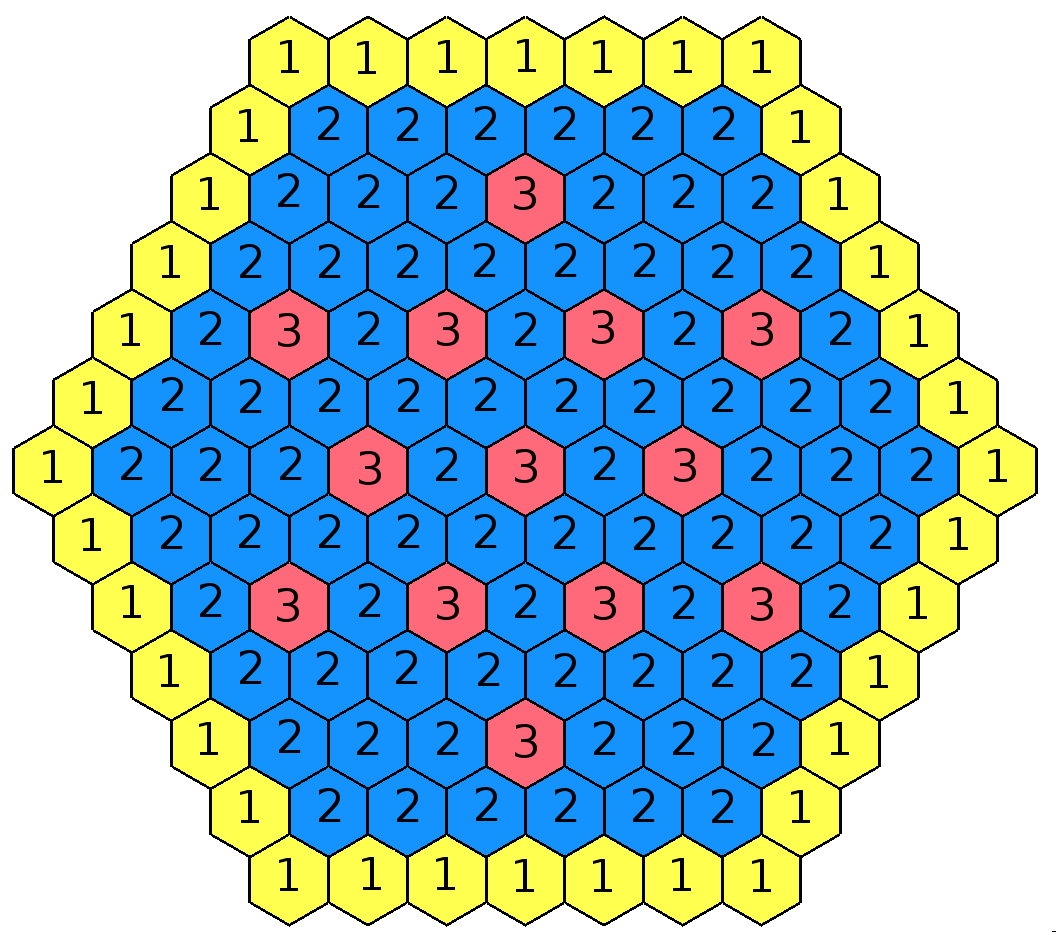
\includegraphics[width=0.48\linewidth] {1.png}
	\caption{Geometrcial model of the IAEA-2D reactor core}
	\label{fig:1}
  \end{center}
\end{figure} 
\begin{table}[ht]
\caption{Diffusion neutronics constants for IAEA-2D test problem}
\label{t-1}
\begin{center}
\begin{tabular}{cccc}
\hline
Zone & 1 & 2 & 3\\
\hline
$D$, cm & 1.03 & 1.03 & 1.03 \\
$\Sigma_a$, cm$^{-1}$ & 0.02 & 0.02125 & 0.02625 \\
$\nu\Sigma_{f}$, cm$^{-1}$ & 0.0225 & 0.0225 & 0.0225\\
\hline
\end{tabular}
\end{center}
\end{table}
Modeling effect of immersion or extraction of control rods (depending on the sign of the perturbation). Define the scenario of process:
\begin{enumerate} 
\item The spectral problem is solved \cite{Annals17}, the solution is taken as the initial condition;
\item Calculation for the non-stationary model in the time range 0 to 0.1 sec;
\item At a moment of 0.1 sec the value $\Sigma_a$ for the zone 3 changes to $\pm$ 0.000625;
\item The dynamic regime is calculated starting from 0.1 sec to 0.5 sec.
\end{enumerate}
At each time the integrated power is calculated 
\[
P(t) = a\int_{\Omega}\Sigma_f \varphi d\bm x,
\]
where $a$ is the normalization coefficient by a given value of the integrated power.

\textbf{Computational results.}
The accuracy of the solution was evaluated by a reference solution, which uses a numerical solution on a sufficiently detailed grid in time
($\tau_{ref} = 1 \cdot 10^{-5}$) by the implicit scheme with a fixed time step. The initial value of $k_{eff}$ was 1.0005063. Figure \ref{fig:2} show the integral powers for the immersion and the extraction of the control rods respectively.

\begin{figure}[ht]
  \begin{center}
    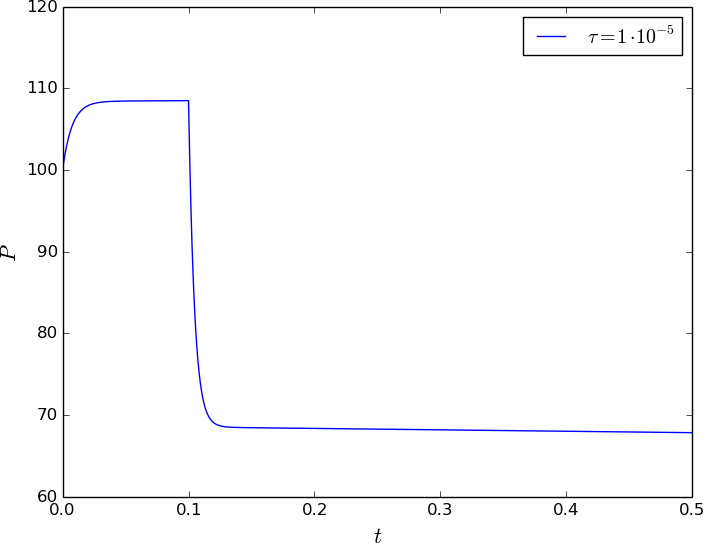
\includegraphics[width=0.48\linewidth] {power_down.png}
    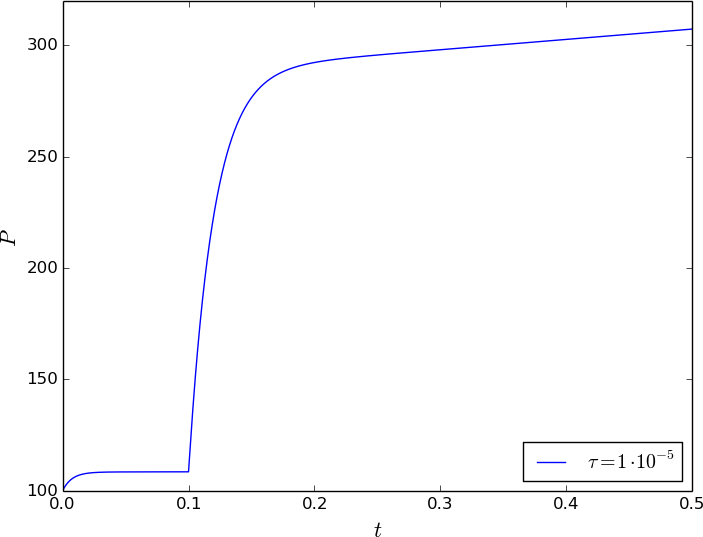
\includegraphics[width=0.48\linewidth] {power_up.png}
	\caption{The integral powers.}
	\label{fig:2}
  \end{center}
\end{figure}

The error is estimated as $\varepsilon_P(t) = |P_{ref} - P|,$
where $P_{ref}$ is the reference solution, $P$ is the solution obtained by using the time stepping algorithm.
We took a minimum time step $\tau_0 = \tau_{ref}$.

Figure \ref{fig:3} show the error $\varepsilon_P$ when the control rods are taken for immersion and extraction, respectively, for different values of the parameter
$\delta$. Here we see that the error converges as the parameter $\delta$ decreases.

\begin{figure}[ht]
  \begin{center}
    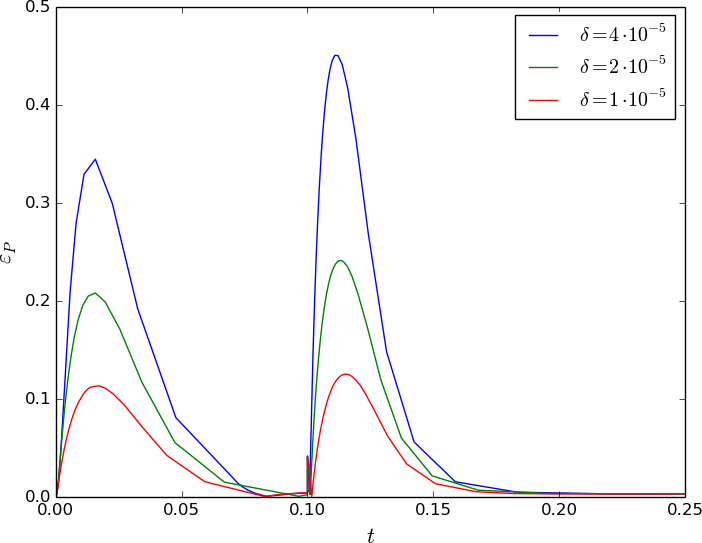
\includegraphics[width=0.48\linewidth] {delta_down.png}
    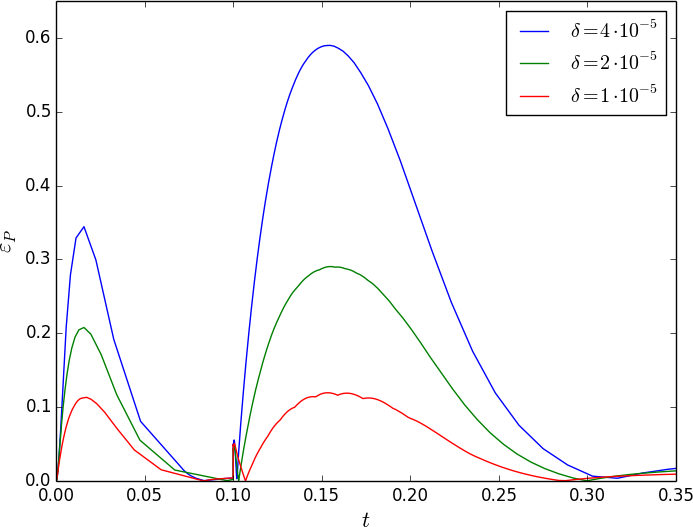
\includegraphics[width=0.48\linewidth] {delta_up.png}
	\caption{Error by time.}
	\label{fig:3}
  \end{center}
\end{figure}

Figure \ref{fig:4} shows the time steps for immersion and extraction rods, respectively. It is seen that first there is a rapid growth of the time step with a specified accuracy of $\delta$.
Then the \textit{catch} of a sudden change in power occurs with a strong decrease in the time step.
Further, the time step grows to a certain point and remains at the same level, which is controlled by the error $\delta$.

\begin{figure}[ht]
  \begin{center}
    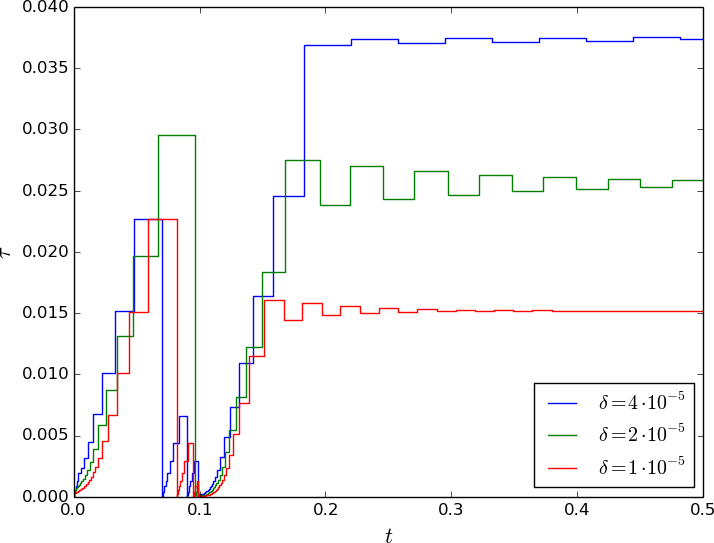
\includegraphics[width=0.48\linewidth] {step_down.png}
    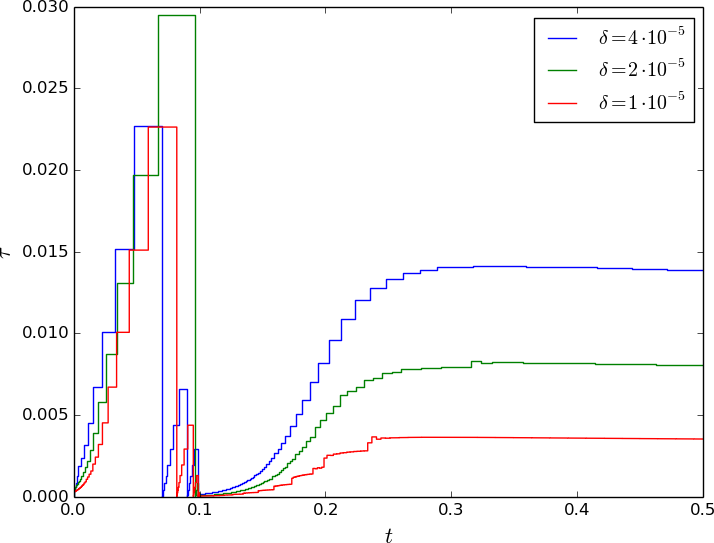
\includegraphics[width=0.48\linewidth] {step_up.png}
    	\caption{Steps by time.}
	\label{fig:4}
  \end{center}
\end{figure} 

Table \ref{t-2} shows the various output data for different values of the parameter $\delta$, where max($\epsilon_P$) is the maximum power error, $n$ is the number of steps in time, and $t$ is the calculation time in seconds.
The reference solution: the number of steps in time is 50000, the counting time is 2130 seconds.
\begin{table}[ht]
\caption{Counting time and number of steps.}
\label{t-2}
\begin{center}
\begin{tabular}{ccrrcrr}
&\multicolumn{3}{c}{immsersion} & \multicolumn{3}{c}{extraction}\\
\hline
$\delta$ & max($\epsilon_P$) & $n$ & $t$, сек & max($\epsilon_P$)  & $n$ & $t$, сек \\
\hline
$4\cdot 10^{-5}$ & 0.450 & 136 & 16 & 0.590 & 241 & 35 \\
$2\cdot 10^{-5}$ & 0.241 & 159 & 20 & 0.290 & 373 & 62 \\
$1\cdot 10^{-5}$ & 0.125 & 270 & 37 & 0.120 & 773 & 145 \\
\hline
\end{tabular}
\end{center}
\end{table}

\section*{Acknowledgements}
This work are supported A.V. Avvakumov and V.F.Strizhov by the Russian Foundation for Basic Research \#16-08-01215, P.N. Vabishchevich by the grant of the Russian Federation Government \#14.Y26.31.0013 and A.O. Vasilev by the Russian Foundation for Basic Research \#18-31-00315.

\begin{thebibliography}{8}
\bibitem{Matus}
Samarskii, ~A.~A., Matus, ~P.~P., Vabishchevich, ~P.~N.: Difference Schemes
  with Operator Factors. Kluwer, (2002)
  
\bibitem{Ascher}
Ascher, ~U.~M.: Computer methods for ordinary differential equations and
  differential-algebraic equations. Society for Industrial Mathematics, (1998)

\bibitem{Vabishchevich}
Vabishchevich, ~P.~N.: A priori estimation of a time step for
  numerically solving parabolic problems. Mathematical Modelling and
  Analysis. \textbf{20}(1), 94--111 (2015)

\bibitem{Matmod}
Avvakumov,~A.~V., et al.: Numerical modeling of neutron diffusion non-stationary problems. Matematicheskoe Modelirovanie.\textbf{29}(7), 44--62 (2017)

\bibitem{Chao}
Chao, ~Y.~A., Shatilla, ~Y.~A.: Conformal mapping and hexagonal nodal methods-II: Implementation in the ANC-H Code. Nuclear Science and Engineering. \textbf{121}, 210--225 (1995)

\bibitem{Annals17}
Avvakumov,~A.~V., et al.: Spectral properties of dynamic processes in a nuclear reactor. Annals of Nuclear Energy. \textbf{99}, 68--79 (2017) 

\bibitem{Lozenets16}
Avvakumov, ~A.~V., et~al.: Algorithms for Numerical Simulation of Non-stationary Neutron Diffusion Problems. In: NAA 2016. pp. 212--219. Springer, Cham (2016)

\end{thebibliography}
\end{document}
